\documentclass{beamer}

\mode<presentation>
 {
% \usetheme{Frankfurt}
 \usecolortheme{fly}
 }

\usepackage[utf8]{inputenc}

\newcommand{\fullframegraphic}[1]{
\begin{frame}[c]
    \includegraphics[height=\textheight,width=\textwidth,keepaspectratio]{#1}
\end{frame}

}

\logo{\includegraphics[height=1cm]{imagenes/FLISoL-2015.png}}

\title{Privacidad en Internet}
%\includegraphics{imagenes/FLISoL-2015.png}
\subtitle{o como perdimos la privacidad}
\author{Lucas Esequiel Bellomo}
\institute{FLISoL Río Cuarto}
\date{Abril 25, 2015}

\AtBeginSection[]
{
\begin{frame}<beamer>
\frametitle{Índice}
\tableofcontents[currentsection]
\end{frame}
}

\begin{document}

% this prints title, author etc.
\begin{frame}
  \titlepage
\end{frame}

\section{1ra parte: Conceptual}

\begin{frame}
  \frametitle{Privacidad}
  \begin{columns}
    \column{.5\textwidth}
    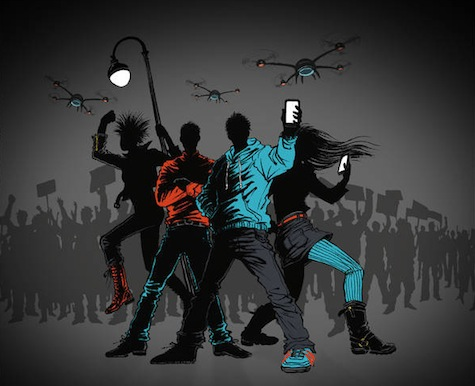
\includegraphics[keepaspectratio=true,width=.35\paperwidth]{imagenes/homeland.jpg}
    \column{.5\textwidth}
     Derecho a la soberanía de tus propios datos (o privacidad)
  \end{columns}
\end{frame}

\begin{frame}
  \frametitle{Distopías}
  \begin{tabular}{cc}
     \includegraphics[keepaspectratio=true,width=.35\paperwidth]{imagenes/1984.jpeg} & \pause \includegraphics[keepaspectratio=true,width=.35\paperwidth]{imagenes/el-proceso.jpeg}
     \end{tabular}
     Basado en presentación Garage Lab de Emiliano Kargieman y Gerardo Richarte
  \end{frame}

\begin{frame}
  \frametitle{1984}
  \begin{columns}
    \column{.5\textwidth}
    \includegraphics[keepaspectratio=true,width=.35\paperwidth]{imagenes/camaras.jpg}
    \column{.5\textwidth}
    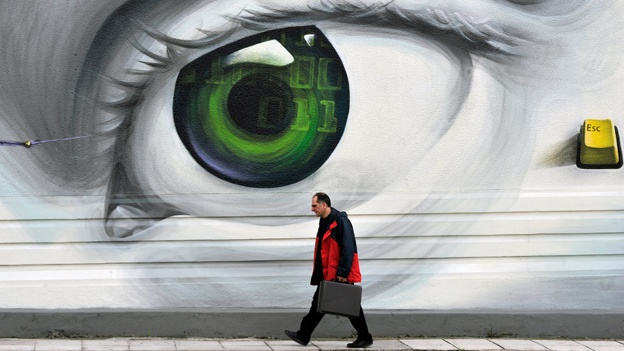
\includegraphics[keepaspectratio=true,width=.55\paperwidth]{imagenes/privacidad_01.jpg}
    \end{columns}
  \begin{itemize}
  \item Estado de vigilancia \pause
  \item Control social \pause
  \item Privaciones a la libertad de expresión \pause
  \item Privaciones a la libertad de pensamiento \pause
  \item Basado en lo que la gente esta haciendo
  \end{itemize}
\end{frame}

\begin{frame}
  \includegraphics[height=\textheight,width=\textwidth,keepaspectratio]{imagenes/cctv.jpg}
\end{frame}


\begin{frame}
   \includegraphics[height=\textheight,width=\textwidth,keepaspectratio]{imagenes/la-plata-camaras-moviles.jpg}
\end{frame}

\begin{frame}
  \frametitle{El Proceso}
  \begin{columns}
    \column{.5\textwidth}
    Una burocracia sin cara toma decisiones significativas sobre las personas, sin que estas tengan control o, aunque sea, opinión.
    \column{.5\textwidth}
    \includegraphics[keepaspectratio=true,width=.35\paperwidth]{imagenes/proceso.jpeg}
  \end{columns}
\end{frame}

\begin{frame}
  \frametitle{El Proceso}
  \begin{columns}
    \column{.5\textwidth}
  \begin{itemize}
  \item Yo no tengo nada que ocultar
  \item Yo no soy un delincuente \pause
    \end{itemize}
    \column{.5\textwidth}
      \begin{tabular}{cc}
         Recolección de información & + \\
         Agregación de datos & + \\
         Procesamiento  \\
         \hline
         Desbalance de poder
    \end{tabular}
    \end{columns}
    \pause
    \begin{block}{ }
    \begin{center}
      "Todo el mundo tiene tres vidas: \\ la pública, la privada y la secreta"
  \end{center}
%  \begin{right}
     \textit{Gabriel García Márquez}
%   \end{right}
     \end{block}
 \end{frame}

\begin{frame}
  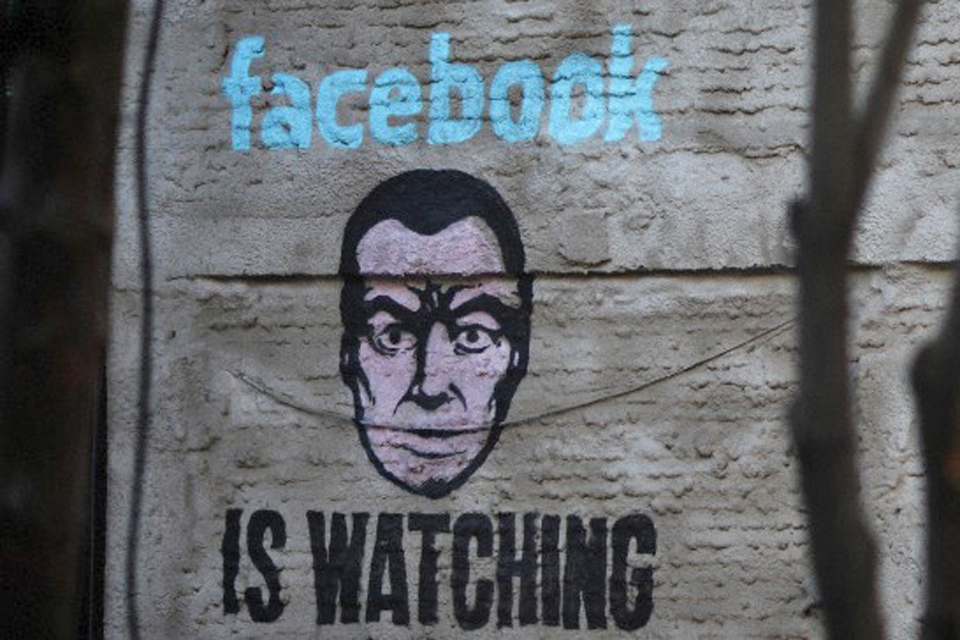
\includegraphics[keepaspectratio=true,width=.8\paperwidth]{imagenes/FB-is_watching.jpg}
  \begin{itemize}
  \item ¡Orwell nunca imaginó que nosotros pondríamos las cámaras!
  \item  Somos los que mantenemos actualizadas las bases de datos (¡y con gusto!)
  \end{itemize}
\end{frame}

\begin{frame}
  \frametitle{¿Cuánto conoce Google sobre nosotros?}
  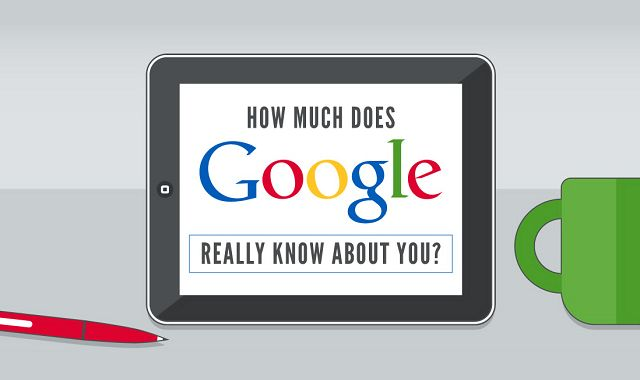
\includegraphics[height=\textheight,width=\textwidth,keepaspectratio]{imagenes/How-Much-Does-Google-Really-Know-About-You.jpg}
\end{frame}

\begin{frame}
    \frametitle{¿Cuánto conoce Google sobre nosotros?}
  \begin{columns}
  \column{.5\textwidth}
  \begin{itemize}
   \item Google Books \pause
   \item Google Docs  \pause
   \item Google   \pause
   \item Google Trends  \pause
   \item Google Analytics  \pause
   \item Youtube  \pause
   \item Google Scholar  \pause
   \item Gmail  \pause
          \item Hangout  \pause
    \end{itemize}
   \column{.5\textwidth}
     \begin{itemize}
       \item Google Calendar  \pause
       \item Google Groups  \pause
       \item Google Maps  \pause
       \item Google Street View  \pause
       \item Picasa  \pause
       \item Latitude  \pause
       \item Blogger  \pause
       \item Chrome  \pause
        \item Android  \pause
         \end{itemize}
  \end{columns}
\begin{center}
  ¿Más?
\end{center}
\end{frame}

\fullframegraphic{imagenes/google_knows.jpeg}

\begin{frame}
  \frametitle{Samsung Smart TV}
 
\includegraphics[keepaspectratio=true,width=.8\paperwidth]{imagenes/samsung-oculus_news.jpg}
\end{frame}

\begin{frame}
  \frametitle{}
   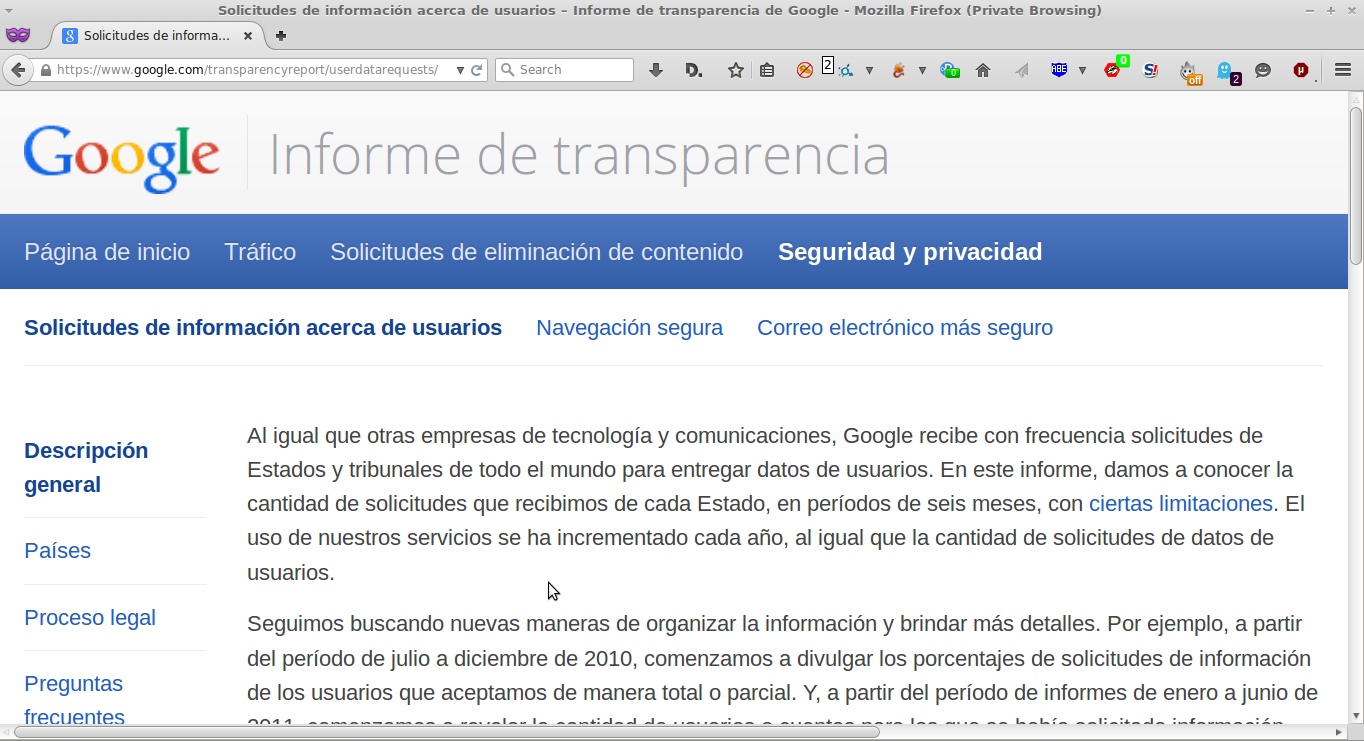
\includegraphics[keepaspectratio=true,width=.8\paperwidth]{imagenes/google_informe_transparencia.png}
\end{frame}

\begin{frame}
  \frametitle{}
  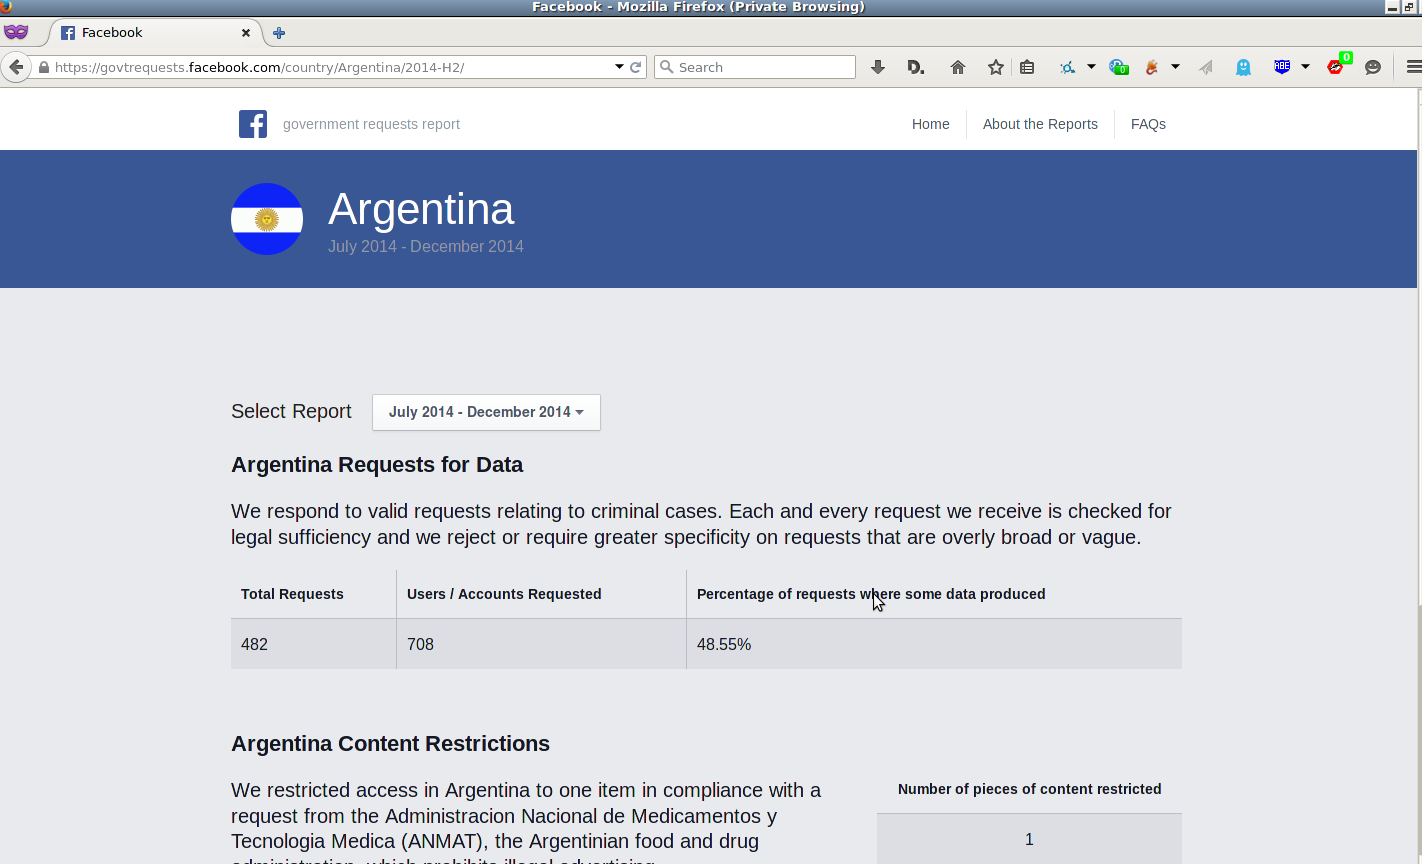
\includegraphics[keepaspectratio=true,width=.8\paperwidth]{imagenes/facebook-government_requests_report.png}
\end{frame}

\fullframegraphic{imagenes/privacidad-muchos_mirando.jpeg}

\section{2da parte: Técnica}

\begin{frame}
  \frametitle{¿Qué podemos hacer?}
    \begin{columns}
    \column{.5\textwidth}
  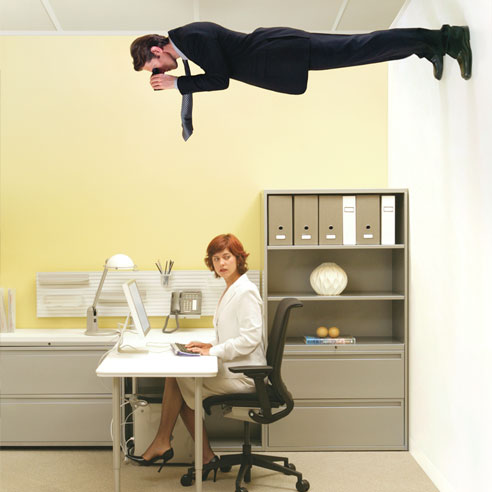
\includegraphics[keepaspectratio=true,width=.5\paperwidth]{imagenes/spying.jpg}
      \column{.5\textwidth}
      \begin{center}
        \textbf{Ser consciente de lo que sucede}
        \end{center}
        \pause
      \begin{itemize}
        \item Herramientas para evitar el tracking
        \item Herramientas para aumentar la seguridad
        \end{itemize}
        \end{columns}
\end{frame}

\begin{frame}
  \frametitle{Extensiones (add-ons) para el navegador}
    \begin{description}[add-ons]
      \item[Privacy Badger] blocks spying ads and invisible trackers
      \item[HTTPS Everywhere] Encrypt the Web! Automatically use HTTPS security on many sites.
      \item[Disconnect]  Make the web faster, more private, and more secure
      \item[Ghostery] Protect your privacy. See who’s tracking your web browsing and block them
      \item[Disconnect+microBlock] para reeplazar Ghostery.
      \item[Blur (o DoNotTrackMe)] Protect your Passwords, Payments, and Privacy
      \item[AdBlock Edge] extension for blocking advertisements on the web.
      \item[Self-Destructing Cookies] Protects against trackers and zombie-cookies
     \end{description}
\end{frame}

\begin{frame}
  \frametitle{Buscadores (más allá de Google)}
  \begin{columns}
        \column{.33\textwidth}
DuckDuckGo  \includegraphics[keepaspectratio=true,width=.25\paperwidth]{imagenes/duckduckgo.jpg}
        \column{.33\textwidth}
StartPage  \includegraphics[keepaspectratio=true,width=.15\paperwidth]{imagenes/sp.jpg}
        \column{.33\textwidth}
        Ixquick \includegraphics[keepaspectratio=true,width=.15\paperwidth]{imagenes/ix.jpeg}
   \end{columns}
\end{frame}


\begin{frame}
  \frametitle{Cuidar la dirección email}
    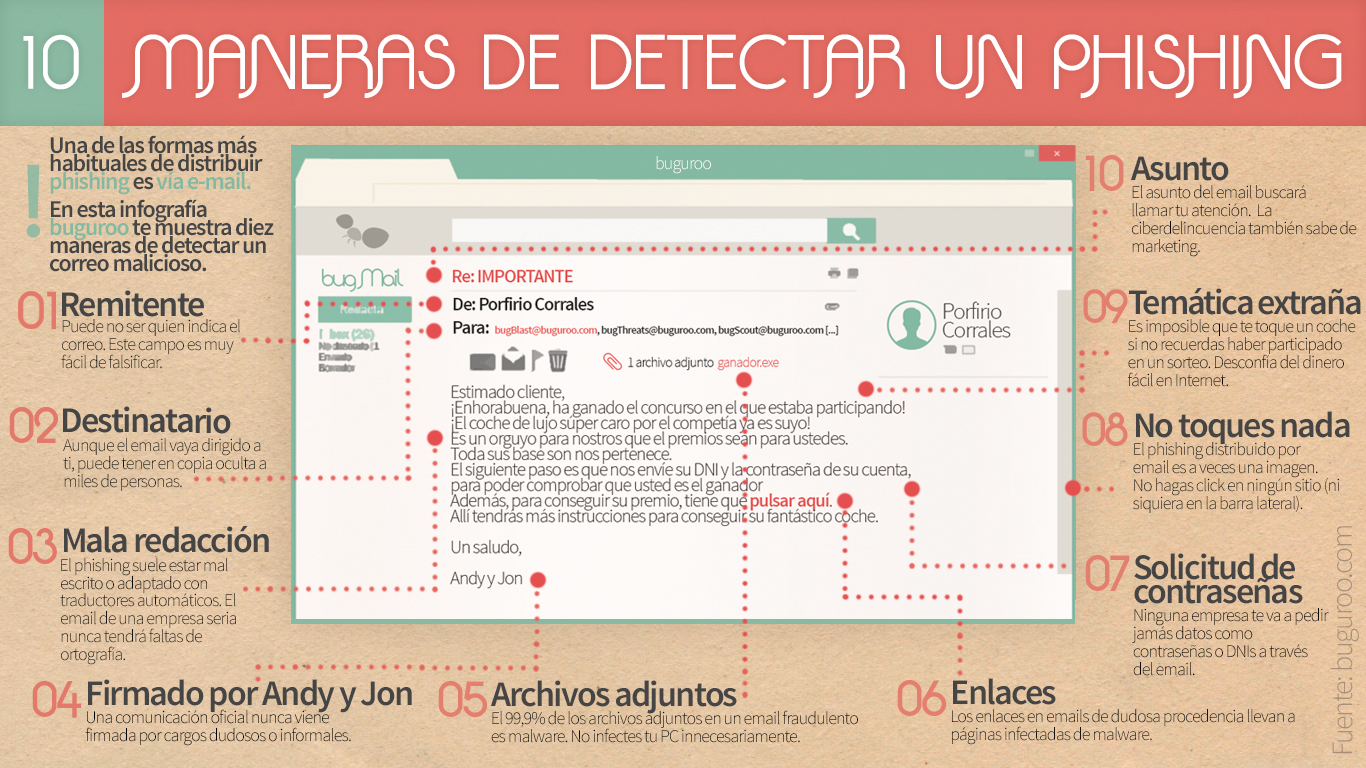
\includegraphics[keepaspectratio=true,width=.8\paperwidth]{imagenes/diez-maneras-detectar-phishing.jpg}
\end{frame}

\begin{frame}
  \frametitle{¿Qué pasó con lavabit?}
\includegraphics[keepaspectratio=true,width=.6\paperwidth]{imagenes/lavabit.png}
\begin{center}
“Me he visto forzado a tomar una difícil decisión: convertirme en cómplice de delitos contra el pueblo estadounidense o dejar al lado casi diez años de duro trabajo y cerrar Lavabit”
\end{center}
\textit{Ladar Levison}
\end{frame}

\begin{frame}
  \frametitle{Email}
  \begin{columns}
    \column{.5\textwidth}
\begin{center}
Alternativas a Gmail
\end{center}
\begin{itemize}
    \item Mantenidos por la comunidad:
      \begin{itemize}
        \item RiseUp
        \item Autistici/Inventati
        \item OpenMailbox 
       \end{itemize}
       \pause
     \item Enfocados en la seguridad desde el diseño
       \begin{itemize}
         \item ProtonMail
         \item Tutanota
         \end{itemize}
       \end{itemize}
       \pause
     \column{.5\textwidth}
\begin{center}
     Encriptar y firmar email
\end{center}
     \begin{tabular}{cc}
       GPG & + \\
       Thunderbird/Claws & + \\
       Enigmail
     \end{tabular}
   \end{columns}
\end{frame}  

\begin{frame}
  \frametitle{Mensajería Instantánea}
  \begin{columns}
    \column{.5\textwidth}
    \begin{center}
      Totalmente seguro no existe \\
      Buenas opciones
    \end{center}
    \begin{itemize}
      \item Pidgin + OTR (Off-the-Record)
      \item Tox
      \item Jabber\XMPP
      \item Cryptocat
    \end{itemize}
    \column{.5\textwidth}
    \begin{center}
      Alternativas a WhatsApp
    \end{center}
    \begin{itemize}
      \item TextSecure
      \item Wickr
      \end{itemize}
      \end{columns}
\end{frame}

\fullframegraphic{imagenes/utox.png}

\begin{frame}
  \frametitle{}
  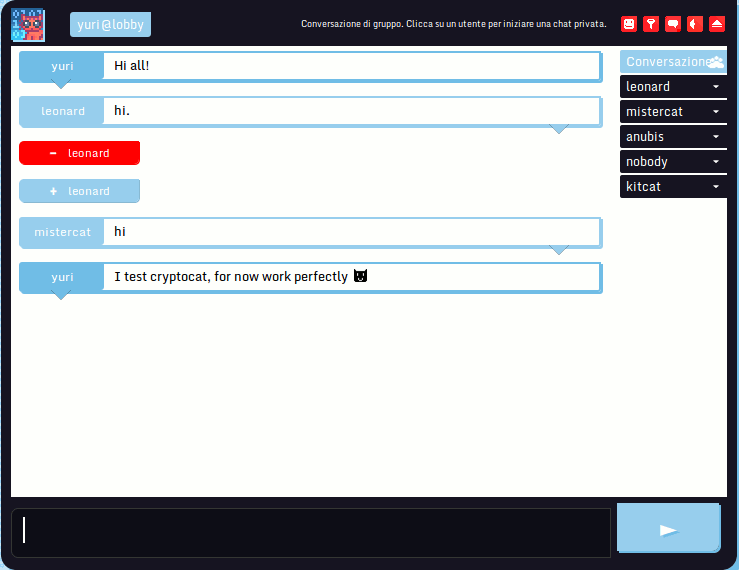
\includegraphics[keepaspectratio=true,width=.7\paperwidth]{imagenes/Cryptocat.png}
\end{frame}

\begin{frame}
  \frametitle{Tor}
  \includegraphics[keepaspectratio=true,width=.7\paperwidth]{imagenes/How_Tor_Works_1.png} 
\end{frame}

\begin{frame}
  \frametitle{Tor}
  \includegraphics[keepaspectratio=true,width=.7\paperwidth]{imagenes/How_Tor_Works_2.png}
\end{frame}

\begin{frame}
  \frametitle{Tor}
  \includegraphics[keepaspectratio=true,width=.7\paperwidth]{imagenes/How_Tor_Works_3.png}
\end{frame}

\begin{frame}
  \frametitle{Referencias}
  \begin{itemize}
  \item \href{https://www.gnu.org/philosophy/surveillance-vs-democracy.es.html}{¿Cuánta vigilancia puede soportar la democracia?}
  \item \href{https://prism-break.org/es/}{PRISM Break}
  \item \href{https://www.eff.org/es/secure-messaging-scorecard}{EFF Secure Messaging Scorecard}
  \item \href{https://www.eff.org/files/2015/03/18/anonimatoycifrado-eff-11.pdf}{Anonimato y cifrado (EFF)}
  \item \href{http://media.espora.org/mgoblin_media/media_entries/1495/Criptotarjetas_RanchoElectronico.pdf}{Cryptotarjetas}
  \item \href{http://www.vialibre.org.ar}{Fundación Vía Libre}
  \item \href{https://www.derechosdigitales.org}{ONG Derechos digitales}
  \item \href{http://www.fundacionsadosky.org.ar/es/programas-proyectos/seguridad-en-tic}{Fundación Sadosky, Programa Seguridad en TIC}
  \item \href{https://ssd.eff.org/es}{Autoprotección Digital Contra La Vigilancia (EFF)}
  \item \href{http://diadeinternet.org/pdfs/Internet_Derechos_Principios.pdf}{Carta de Derechos Humanos y Principios en Internet}
  \item \href{http://www.visualistan.com/2015/02/how-much-does-google-really-know-about-you.html}{how much does google really know about you? (infografía)}
  \item \href{http://www.scoop.it/IPcontrol}
{Breve compendio de noticias e info}  
\item \href{http://derechoaleer.org}{Derecho a Leer}
  \end{itemize}
\end{frame}  
 

\begin{frame}
  \frametitle{Referencias: Charlas}
  \begin{itemize}
    \item \href{https://www.youtube.com/watch?v=lCQ_GA1nmtk}{Beatriz Busaniche sobre la cultura, la privacidad y los derechos en Internet}
      \item \href{http://www.ted.com/talks/andy_yen_think_your_email_s_private_think_again}{Think your email's private? Think again (ProtonMail)}
  \item \href{https://vimeo.com/10965423}{Gerardo Richarte *(Gera)* en GarageLab 4 Post-Privacidad}
 \item \href{https://www.youtube.com/watch?v=tnDxRjMDGQM}{¿Cómo nos vigilan en internet?}
\end{itemize}
\end{frame}  

\begin{frame}
  \frametitle{Agradecimientos}
  \begin{itemize}
\item Iván Arce
\item Maximiliano Giraldes
\item Enrique Chaparro
\item Tess
\item @derechoaleer
\item Evelin Heidel
\item Teresa Sempere García
\item Pascual Calicchio
\item @PirataCland
\end{itemize}

\begin{center}
\includegraphics[keepaspectratio=true,width=.3\paperwidth]{imagenes/it10.png}
\end{center}
\end{frame}

\begin{frame}
\frametitle{Licencia}
\begin{center}
This work is licensed under a Creative Commons Attribution 4.0 International License. \\

\includegraphics[keepaspectratio=true,width=.3\paperwidth]{imagenes/CC_BY.png}
\end{center}
\end{frame}

\begin{frame}
\begin{center}
¡Gracias por su atención!
\end{center}
\end{frame}

\end{document}